\documentclass[1p]{elsarticle_modified}
%\bibliographystyle{elsarticle-num}

%\usepackage[colorlinks]{hyperref}
%\usepackage{abbrmath_seonhwa} %\Abb, \Ascr, \Acal ,\Abf, \Afrak
\usepackage{amsfonts}
\usepackage{amssymb}
\usepackage{amsmath}
\usepackage{amsthm}
\usepackage{scalefnt}
\usepackage{amsbsy}
\usepackage{kotex}
\usepackage{caption}
\usepackage{subfig}
\usepackage{color}
\usepackage{graphicx}
\usepackage{xcolor} %% white, black, red, green, blue, cyan, magenta, yellow
\usepackage{float}
\usepackage{setspace}
\usepackage{hyperref}

\usepackage{tikz}
\usetikzlibrary{arrows}

\usepackage{multirow}
\usepackage{array} % fixed length table
\usepackage{hhline}

%%%%%%%%%%%%%%%%%%%%%
\makeatletter
\renewcommand*\env@matrix[1][\arraystretch]{%
	\edef\arraystretch{#1}%
	\hskip -\arraycolsep
	\let\@ifnextchar\new@ifnextchar
	\array{*\c@MaxMatrixCols c}}
\makeatother %https://tex.stackexchange.com/questions/14071/how-can-i-increase-the-line-spacing-in-a-matrix
%%%%%%%%%%%%%%%

\usepackage[normalem]{ulem}

\newcommand{\msout}[1]{\ifmmode\text{\sout{\ensuremath{#1}}}\else\sout{#1}\fi}
%SOURCE: \msout is \stkout macro in https://tex.stackexchange.com/questions/20609/strikeout-in-math-mode

\newcommand{\cancel}[1]{
	\ifmmode
	{\color{red}\msout{#1}}
	\else
	{\color{red}\sout{#1}}
	\fi
}

\newcommand{\add}[1]{
	{\color{blue}\uwave{#1}}
}

\newcommand{\replace}[2]{
	\ifmmode
	{\color{red}\msout{#1}}{\color{blue}\uwave{#2}}
	\else
	{\color{red}\sout{#1}}{\color{blue}\uwave{#2}}
	\fi
}

\newcommand{\Sol}{\mathcal{S}} %segment
\newcommand{\D}{D} %diagram
\newcommand{\A}{\mathcal{A}} %arc


%%%%%%%%%%%%%%%%%%%%%%%%%%%%%5 test

\def\sl{\operatorname{\textup{SL}}(2,\Cbb)}
\def\psl{\operatorname{\textup{PSL}}(2,\Cbb)}
\def\quan{\mkern 1mu \triangleright \mkern 1mu}

\theoremstyle{definition}
\newtheorem{thm}{Theorem}[section]
\newtheorem{prop}[thm]{Proposition}
\newtheorem{lem}[thm]{Lemma}
\newtheorem{ques}[thm]{Question}
\newtheorem{cor}[thm]{Corollary}
\newtheorem{defn}[thm]{Definition}
\newtheorem{exam}[thm]{Example}
\newtheorem{rmk}[thm]{Remark}
\newtheorem{alg}[thm]{Algorithm}

\newcommand{\I}{\sqrt{-1}}
\begin{document}

%\begin{frontmatter}
%
%\title{Boundary parabolic representations of knots up to 8 crossings}
%
%%% Group authors per affiliation:
%\author{Yunhi Cho} 
%\address{Department of Mathematics, University of Seoul, Seoul, Korea}
%\ead{yhcho@uos.ac.kr}
%
%
%\author{Seonhwa Kim} %\fnref{s_kim}}
%\address{Center for Geometry and Physics, Institute for Basic Science, Pohang, 37673, Korea}
%\ead{ryeona17@ibs.re.kr}
%
%\author{Hyuk Kim}
%\address{Department of Mathematical Sciences, Seoul National University, Seoul 08826, Korea}
%\ead{hyukkim@snu.ac.kr}
%
%\author{Seokbeom Yoon}
%\address{Department of Mathematical Sciences, Seoul National University, Seoul, 08826,  Korea}
%\ead{sbyoon15@snu.ac.kr}
%
%\begin{abstract}
%We find all boundary parabolic representation of knots up to 8 crossings.
%
%\end{abstract}
%\begin{keyword}
%    \MSC[2010] 57M25 
%\end{keyword}
%
%\end{frontmatter}

%\linenumbers
%\tableofcontents
%
\newcommand\colored[1]{\textcolor{white}{\rule[-0.35ex]{0.8em}{1.4ex}}\kern-0.8em\color{red} #1}%
%\newcommand\colored[1]{\textcolor{white}{ #1}\kern-2.17ex	\textcolor{white}{ #1}\kern-1.81ex	\textcolor{white}{ #1}\kern-2.15ex\color{red}#1	}

{\Large $\underline{11a_{174}~(K11a_{174})}$}

\setlength{\tabcolsep}{10pt}
\renewcommand{\arraystretch}{1.6}
\vspace{1cm}\begin{tabular}{m{100pt}>{\centering\arraybackslash}m{274pt}}
\multirow{5}{120pt}{
	\centering
	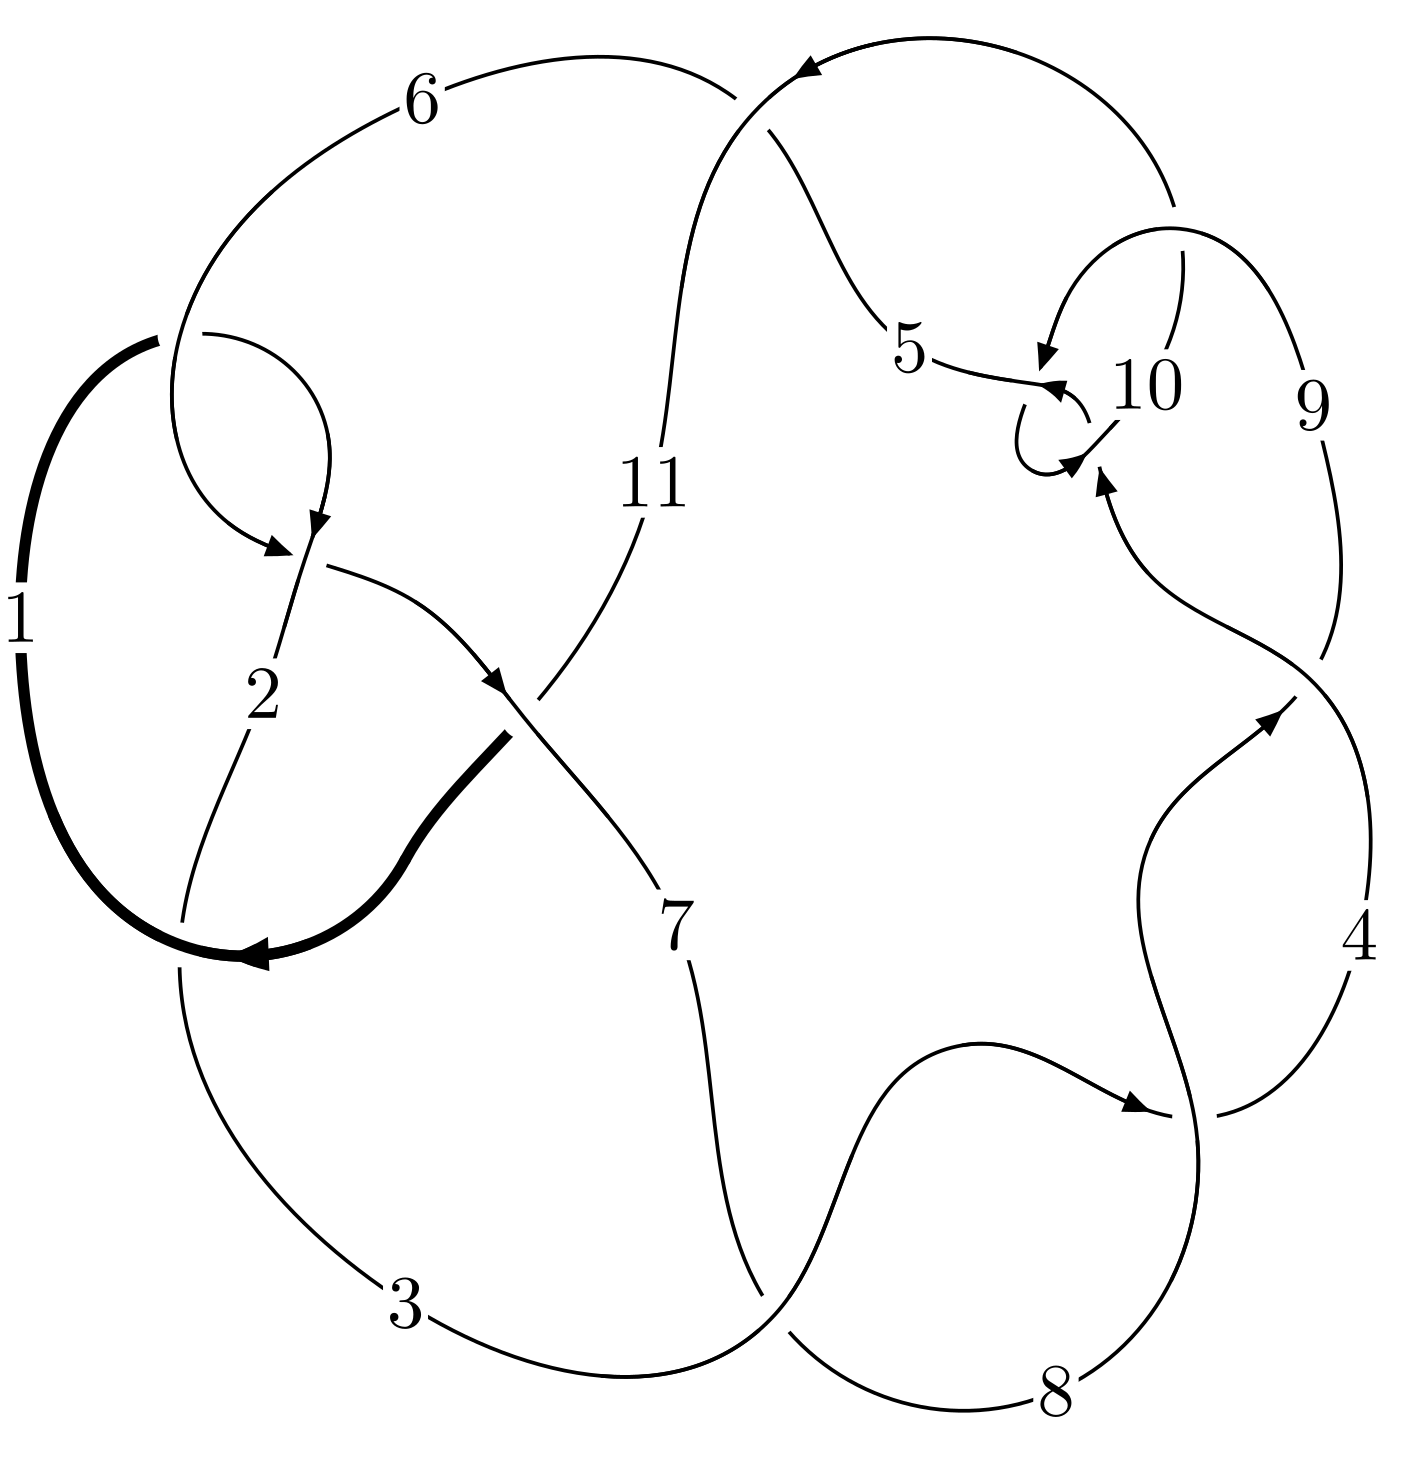
\includegraphics[width=112pt]{../../../GIT/diagram.site/Diagrams/png/423_11a_174.png}\\
\ \ \ A knot diagram\footnotemark}&
\allowdisplaybreaks
\textbf{Linearized knot diagam} \\
\cline{2-2}
 &
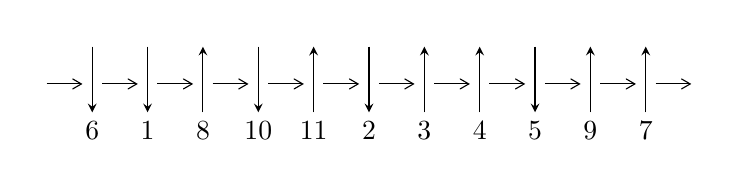
\begin{tikzpicture}[x=20pt, y=17pt]
	% nodes
	\node (C0) at (0, 0) {};
	\node (C1) at (1, 0) {};
	\node (C1U) at (1, +1) {};
	\node (C1D) at (1, -1) {6};

	\node (C2) at (2, 0) {};
	\node (C2U) at (2, +1) {};
	\node (C2D) at (2, -1) {1};

	\node (C3) at (3, 0) {};
	\node (C3U) at (3, +1) {};
	\node (C3D) at (3, -1) {8};

	\node (C4) at (4, 0) {};
	\node (C4U) at (4, +1) {};
	\node (C4D) at (4, -1) {10};

	\node (C5) at (5, 0) {};
	\node (C5U) at (5, +1) {};
	\node (C5D) at (5, -1) {11};

	\node (C6) at (6, 0) {};
	\node (C6U) at (6, +1) {};
	\node (C6D) at (6, -1) {2};

	\node (C7) at (7, 0) {};
	\node (C7U) at (7, +1) {};
	\node (C7D) at (7, -1) {3};

	\node (C8) at (8, 0) {};
	\node (C8U) at (8, +1) {};
	\node (C8D) at (8, -1) {4};

	\node (C9) at (9, 0) {};
	\node (C9U) at (9, +1) {};
	\node (C9D) at (9, -1) {5};

	\node (C10) at (10, 0) {};
	\node (C10U) at (10, +1) {};
	\node (C10D) at (10, -1) {9};

	\node (C11) at (11, 0) {};
	\node (C11U) at (11, +1) {};
	\node (C11D) at (11, -1) {7};
	\node (C12) at (12, 0) {};

	% arrows
	\draw[->,>={angle 60}]
	(C0) edge (C1) (C1) edge (C2) (C2) edge (C3) (C3) edge (C4) (C4) edge (C5) (C5) edge (C6) (C6) edge (C7) (C7) edge (C8) (C8) edge (C9) (C9) edge (C10) (C10) edge (C11) (C11) edge (C12) ;	\draw[->,>=stealth]
	(C1U) edge (C1D) (C2U) edge (C2D) (C3D) edge (C3U) (C4U) edge (C4D) (C5D) edge (C5U) (C6U) edge (C6D) (C7D) edge (C7U) (C8D) edge (C8U) (C9U) edge (C9D) (C10D) edge (C10U) (C11D) edge (C11U) ;
	\end{tikzpicture} \\
\hhline{~~} \\& 
\textbf{Solving Sequence} \\ \cline{2-2} 
 &
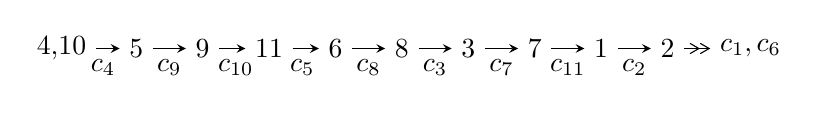
\begin{tikzpicture}[x=24pt, y=7pt]
	% node
	\node (A0) at (-1/8, 0) {4,10};
	\node (A1) at (1, 0) {5};
	\node (A2) at (2, 0) {9};
	\node (A3) at (3, 0) {11};
	\node (A4) at (4, 0) {6};
	\node (A5) at (5, 0) {8};
	\node (A6) at (6, 0) {3};
	\node (A7) at (7, 0) {7};
	\node (A8) at (8, 0) {1};
	\node (A9) at (9, 0) {2};
	\node (C1) at (1/2, -1) {$c_{4}$};
	\node (C2) at (3/2, -1) {$c_{9}$};
	\node (C3) at (5/2, -1) {$c_{10}$};
	\node (C4) at (7/2, -1) {$c_{5}$};
	\node (C5) at (9/2, -1) {$c_{8}$};
	\node (C6) at (11/2, -1) {$c_{3}$};
	\node (C7) at (13/2, -1) {$c_{7}$};
	\node (C8) at (15/2, -1) {$c_{11}$};
	\node (C9) at (17/2, -1) {$c_{2}$};
	\node (A10) at (41/4, 0) {$c_{1},c_{6}$};

	% edge
	\draw[->,>=stealth]	
	(A0) edge (A1) (A1) edge (A2) (A2) edge (A3) (A3) edge (A4) (A4) edge (A5) (A5) edge (A6) (A6) edge (A7) (A7) edge (A8) (A8) edge (A9) ;
	\draw[->>,>={angle 60}]	
	(A9) edge (A10);
\end{tikzpicture} \\ 

\end{tabular} \\

\footnotetext{
The image of knot diagram is generated by the software ``\textbf{Draw programme}" developed by Andrew Bartholomew(\url{http://www.layer8.co.uk/maths/draw/index.htm\#Running-draw}), where we modified some parts for our purpose(\url{https://github.com/CATsTAILs/LinksPainter}).
}\phantom \\ \newline 
\centering \textbf{Ideals for irreducible components\footnotemark of $X_{\text{par}}$} 
 
\begin{align*}
I^u_{1}&=\langle 
u^{39}- u^{38}+\cdots+2 u^3-1\rangle \\
\\
\end{align*}
\raggedright * 1 irreducible components of $\dim_{\mathbb{C}}=0$, with total 39 representations.\\
\footnotetext{All coefficients of polynomials are rational numbers. But the coefficients are sometimes approximated in decimal forms when there is not enough margin.}
\newpage
\renewcommand{\arraystretch}{1}
\centering \section*{I. $I^u_{1}= \langle u^{39}- u^{38}+\cdots+2 u^3-1 \rangle$}
\flushleft \textbf{(i) Arc colorings}\\
\begin{tabular}{m{7pt} m{180pt} m{7pt} m{180pt} }
\flushright $a_{4}=$&$\begin{pmatrix}1\\0\end{pmatrix}$ \\
\flushright $a_{10}=$&$\begin{pmatrix}0\\u\end{pmatrix}$ \\
\flushright $a_{5}=$&$\begin{pmatrix}1\\u^2\end{pmatrix}$ \\
\flushright $a_{9}=$&$\begin{pmatrix}u\\u^3+u\end{pmatrix}$ \\
\flushright $a_{11}=$&$\begin{pmatrix}u^3\\u^5+u^3+u\end{pmatrix}$ \\
\flushright $a_{6}=$&$\begin{pmatrix}- u^6- u^4+1\\- u^8-2 u^6-2 u^4\end{pmatrix}$ \\
\flushright $a_{8}=$&$\begin{pmatrix}- u^3\\u^3+u\end{pmatrix}$ \\
\flushright $a_{3}=$&$\begin{pmatrix}- u^6- u^4+1\\u^6+2 u^4+u^2\end{pmatrix}$ \\
\flushright $a_{7}=$&$\begin{pmatrix}u^9+2 u^7+u^5-2 u^3- u\\- u^9-3 u^7-3 u^5+u\end{pmatrix}$ \\
\flushright $a_{1}=$&$\begin{pmatrix}u^{23}+6 u^{21}+\cdots+6 u^5+2 u^3\\- u^{23}-7 u^{21}+\cdots-3 u^5+u\end{pmatrix}$ \\
\flushright $a_{2}=$&$\begin{pmatrix}u^{37}+10 u^{35}+\cdots+2 u^3- u\\u^{38}- u^{37}+\cdots+u+1\end{pmatrix}$\\ \flushright $a_{2}=$&$\begin{pmatrix}u^{37}+10 u^{35}+\cdots+2 u^3- u\\u^{38}- u^{37}+\cdots+u+1\end{pmatrix}$\\&\end{tabular}
\flushleft \textbf{(ii) Obstruction class $= -1$}\\~\\
\flushleft \textbf{(iii) Cusp Shapes $= -4 u^{37}+4 u^{36}-44 u^{35}+40 u^{34}-228 u^{33}+192 u^{32}-708 u^{31}+556 u^{30}-1396 u^{29}+1024 u^{28}-1636 u^{27}+1100 u^{26}-628 u^{25}+284 u^{24}+1308 u^{23}-1084 u^{22}+2424 u^{21}-1760 u^{20}+1512 u^{19}-1012 u^{18}-320 u^{17}+300 u^{16}-1080 u^{15}+804 u^{14}-528 u^{13}+396 u^{12}+92 u^{11}-44 u^{10}+132 u^9-92 u^8-16 u^7-12 u^6-36 u^5+8 u^4+4 u^3+4 u^2+4 u+2$}\\~\\
\newpage\renewcommand{\arraystretch}{1}
\flushleft \textbf{(iv) u-Polynomials at the component}\newline \\
\begin{tabular}{m{50pt}|m{274pt}}
Crossings & \hspace{64pt}u-Polynomials at each crossing \\
\hline $$\begin{aligned}c_{1},c_{6}\end{aligned}$$&$\begin{aligned}
&u^{39}- u^{38}+\cdots+2 u-1
\end{aligned}$\\
\hline $$\begin{aligned}c_{2}\end{aligned}$$&$\begin{aligned}
&u^{39}+17 u^{38}+\cdots+2 u^2+1
\end{aligned}$\\
\hline $$\begin{aligned}c_{3},c_{5},c_{7}\\c_{8}\end{aligned}$$&$\begin{aligned}
&u^{39}+u^{38}+\cdots+14 u-1
\end{aligned}$\\
\hline $$\begin{aligned}c_{4},c_{9}\end{aligned}$$&$\begin{aligned}
&u^{39}- u^{38}+\cdots+2 u^3-1
\end{aligned}$\\
\hline $$\begin{aligned}c_{10}\end{aligned}$$&$\begin{aligned}
&u^{39}-23 u^{38}+\cdots-2 u^2+1
\end{aligned}$\\
\hline $$\begin{aligned}c_{11}\end{aligned}$$&$\begin{aligned}
&u^{39}-3 u^{38}+\cdots-14 u+3
\end{aligned}$\\
\hline
\end{tabular}\\~\\
\newpage\renewcommand{\arraystretch}{1}
\flushleft \textbf{(v) Riley Polynomials at the component}\newline \\
\begin{tabular}{m{50pt}|m{274pt}}
Crossings & \hspace{64pt}Riley Polynomials at each crossing \\
\hline $$\begin{aligned}c_{1},c_{6}\end{aligned}$$&$\begin{aligned}
&y^{39}-17 y^{38}+\cdots-2 y^2-1
\end{aligned}$\\
\hline $$\begin{aligned}c_{2}\end{aligned}$$&$\begin{aligned}
&y^{39}+11 y^{38}+\cdots-4 y-1
\end{aligned}$\\
\hline $$\begin{aligned}c_{3},c_{5},c_{7}\\c_{8}\end{aligned}$$&$\begin{aligned}
&y^{39}-49 y^{38}+\cdots+96 y-1
\end{aligned}$\\
\hline $$\begin{aligned}c_{4},c_{9}\end{aligned}$$&$\begin{aligned}
&y^{39}+23 y^{38}+\cdots+2 y^2-1
\end{aligned}$\\
\hline $$\begin{aligned}c_{10}\end{aligned}$$&$\begin{aligned}
&y^{39}-13 y^{38}+\cdots+4 y-1
\end{aligned}$\\
\hline $$\begin{aligned}c_{11}\end{aligned}$$&$\begin{aligned}
&y^{39}-5 y^{38}+\cdots+64 y-9
\end{aligned}$\\
\hline
\end{tabular}\\~\\
\newpage\flushleft \textbf{(vi) Complex Volumes and Cusp Shapes}
$$\begin{array}{c|c|c}  
\text{Solutions to }I^u_{1}& \I (\text{vol} + \sqrt{-1}CS) & \text{Cusp shape}\\
 \hline 
\begin{aligned}
u &= -0.071922 + 0.993246 I\end{aligned}
 & \phantom{-}1.71946 + 2.04419 I & \phantom{-}8.16431 - 3.89320 I \\ \hline\begin{aligned}
u &= -0.071922 - 0.993246 I\end{aligned}
 & \phantom{-}1.71946 - 2.04419 I & \phantom{-}8.16431 + 3.89320 I \\ \hline\begin{aligned}
u &= \phantom{-}0.435411 + 0.809083 I\end{aligned}
 & -1.87228 - 5.10221 I & -1.97486 + 8.58209 I \\ \hline\begin{aligned}
u &= \phantom{-}0.435411 - 0.809083 I\end{aligned}
 & -1.87228 + 5.10221 I & -1.97486 - 8.58209 I \\ \hline\begin{aligned}
u &= -0.909371 + 0.016687 I\end{aligned}
 & \phantom{-}10.31070 - 1.71289 I & \phantom{-}5.85984 + 0.15979 I \\ \hline\begin{aligned}
u &= -0.909371 - 0.016687 I\end{aligned}
 & \phantom{-}10.31070 + 1.71289 I & \phantom{-}5.85984 - 0.15979 I \\ \hline\begin{aligned}
u &= \phantom{-}0.908911 + 0.030266 I\end{aligned}
 & \phantom{-}8.53389 + 7.14392 I & \phantom{-}3.38402 - 4.70933 I \\ \hline\begin{aligned}
u &= \phantom{-}0.908911 - 0.030266 I\end{aligned}
 & \phantom{-}8.53389 - 7.14392 I & \phantom{-}3.38402 + 4.70933 I \\ \hline\begin{aligned}
u &= -0.411819 + 1.010030 I\end{aligned}
 & \phantom{-}0.09606 + 2.71206 I & \phantom{-}0.59234 - 4.52974 I \\ \hline\begin{aligned}
u &= -0.411819 - 1.010030 I\end{aligned}
 & \phantom{-}0.09606 - 2.71206 I & \phantom{-}0.59234 + 4.52974 I \\ \hline\begin{aligned}
u &= \phantom{-}0.880484\phantom{ +0.000000I}\end{aligned}
 & \phantom{-}4.53816\phantom{ +0.000000I} & -0.00697750\phantom{ +0.000000I} \\ \hline\begin{aligned}
u &= -0.305665 + 0.802271 I\end{aligned}
 & \phantom{-}0.32922 + 1.44532 I & \phantom{-}2.59215 - 4.77277 I \\ \hline\begin{aligned}
u &= -0.305665 - 0.802271 I\end{aligned}
 & \phantom{-}0.32922 - 1.44532 I & \phantom{-}2.59215 + 4.77277 I \\ \hline\begin{aligned}
u &= -0.293342 + 1.133220 I\end{aligned}
 & \phantom{-}3.74981 - 2.16888 I & \phantom{-}7.25820 + 2.13079 I \\ \hline\begin{aligned}
u &= -0.293342 - 1.133220 I\end{aligned}
 & \phantom{-}3.74981 + 2.16888 I & \phantom{-}7.25820 - 2.13079 I \\ \hline\begin{aligned}
u &= \phantom{-}0.342277 + 1.124620 I\end{aligned}
 & \phantom{-}5.04615 - 2.65347 I & \phantom{-}9.41633 + 3.85440 I \\ \hline\begin{aligned}
u &= \phantom{-}0.342277 - 1.124620 I\end{aligned}
 & \phantom{-}5.04615 + 2.65347 I & \phantom{-}9.41633 - 3.85440 I \\ \hline\begin{aligned}
u &= \phantom{-}0.429374 + 1.097570 I\end{aligned}
 & \phantom{-}4.38863 - 4.56519 I & \phantom{-}7.75323 + 4.92219 I \\ \hline\begin{aligned}
u &= \phantom{-}0.429374 - 1.097570 I\end{aligned}
 & \phantom{-}4.38863 + 4.56519 I & \phantom{-}7.75323 - 4.92219 I \\ \hline\begin{aligned}
u &= -0.464708 + 1.087840 I\end{aligned}
 & \phantom{-}2.47286 + 9.36763 I & \phantom{-}4.01171 - 9.56282 I \\ \hline\begin{aligned}
u &= -0.464708 - 1.087840 I\end{aligned}
 & \phantom{-}2.47286 - 9.36763 I & \phantom{-}4.01171 + 9.56282 I \\ \hline\begin{aligned}
u &= \phantom{-}0.415674 + 0.642054 I\end{aligned}
 & -2.32655 + 1.37512 I & -4.12538 - 0.53412 I \\ \hline\begin{aligned}
u &= \phantom{-}0.415674 - 0.642054 I\end{aligned}
 & -2.32655 - 1.37512 I & -4.12538 + 0.53412 I \\ \hline\begin{aligned}
u &= -0.632416 + 0.199765 I\end{aligned}
 & -0.01291 - 5.16822 I & \phantom{-}0.66391 + 6.04707 I \\ \hline\begin{aligned}
u &= -0.632416 - 0.199765 I\end{aligned}
 & -0.01291 + 5.16822 I & \phantom{-}0.66391 - 6.04707 I \\ \hline\begin{aligned}
u &= \phantom{-}0.467898 + 1.254570 I\end{aligned}
 & \phantom{-}8.33752 - 4.79855 I & \phantom{-}3.23494 + 3.06059 I \\ \hline\begin{aligned}
u &= \phantom{-}0.467898 - 1.254570 I\end{aligned}
 & \phantom{-}8.33752 + 4.79855 I & \phantom{-}3.23494 - 3.06059 I \\ \hline\begin{aligned}
u &= \phantom{-}0.454344 + 1.275250 I\end{aligned}
 & \phantom{-}12.54280 + 2.32319 I & \phantom{-}6.85027 - 1.71176 I \\ \hline\begin{aligned}
u &= \phantom{-}0.454344 - 1.275250 I\end{aligned}
 & \phantom{-}12.54280 - 2.32319 I & \phantom{-}6.85027 + 1.71176 I \\ \hline\begin{aligned}
u &= \phantom{-}0.488216 + 1.263380 I\end{aligned}
 & \phantom{-}12.2898 - 12.1343 I & \phantom{-}6.37996 + 7.62883 I\\
 \hline 
 \end{array}$$\newpage$$\begin{array}{c|c|c}  
\text{Solutions to }I^u_{1}& \I (\text{vol} + \sqrt{-1}CS) & \text{Cusp shape}\\
 \hline 
\begin{aligned}
u &= \phantom{-}0.488216 - 1.263380 I\end{aligned}
 & \phantom{-}12.2898 + 12.1343 I & \phantom{-}6.37996 - 7.62883 I \\ \hline\begin{aligned}
u &= -0.462613 + 1.273220 I\end{aligned}
 & \phantom{-}14.2633 + 3.1512 I & \phantom{-}9.14562 - 2.87617 I \\ \hline\begin{aligned}
u &= -0.462613 - 1.273220 I\end{aligned}
 & \phantom{-}14.2633 - 3.1512 I & \phantom{-}9.14562 + 2.87617 I \\ \hline\begin{aligned}
u &= -0.481297 + 1.266520 I\end{aligned}
 & \phantom{-}14.1233 + 6.6701 I & \phantom{-}8.91783 - 3.16828 I \\ \hline\begin{aligned}
u &= -0.481297 - 1.266520 I\end{aligned}
 & \phantom{-}14.1233 - 6.6701 I & \phantom{-}8.91783 + 3.16828 I \\ \hline\begin{aligned}
u &= \phantom{-}0.599274 + 0.105705 I\end{aligned}
 & \phantom{-}1.67499 + 0.65150 I & \phantom{-}4.60786 - 0.90927 I \\ \hline\begin{aligned}
u &= \phantom{-}0.599274 - 0.105705 I\end{aligned}
 & \phantom{-}1.67499 - 0.65150 I & \phantom{-}4.60786 + 0.90927 I \\ \hline\begin{aligned}
u &= -0.448469 + 0.341157 I\end{aligned}
 & -1.70724 + 0.92516 I & -3.72881 - 0.98147 I \\ \hline\begin{aligned}
u &= -0.448469 - 0.341157 I\end{aligned}
 & -1.70724 - 0.92516 I & -3.72881 + 0.98147 I\\
 \hline 
 \end{array}$$\newpage
\newpage\renewcommand{\arraystretch}{1}
\centering \section*{ II. u-Polynomials}
\begin{tabular}{m{50pt}|m{274pt}}
Crossings & \hspace{64pt}u-Polynomials at each crossing \\
\hline $$\begin{aligned}c_{1},c_{6}\end{aligned}$$&$\begin{aligned}
&u^{39}- u^{38}+\cdots+2 u-1
\end{aligned}$\\
\hline $$\begin{aligned}c_{2}\end{aligned}$$&$\begin{aligned}
&u^{39}+17 u^{38}+\cdots+2 u^2+1
\end{aligned}$\\
\hline $$\begin{aligned}c_{3},c_{5},c_{7}\\c_{8}\end{aligned}$$&$\begin{aligned}
&u^{39}+u^{38}+\cdots+14 u-1
\end{aligned}$\\
\hline $$\begin{aligned}c_{4},c_{9}\end{aligned}$$&$\begin{aligned}
&u^{39}- u^{38}+\cdots+2 u^3-1
\end{aligned}$\\
\hline $$\begin{aligned}c_{10}\end{aligned}$$&$\begin{aligned}
&u^{39}-23 u^{38}+\cdots-2 u^2+1
\end{aligned}$\\
\hline $$\begin{aligned}c_{11}\end{aligned}$$&$\begin{aligned}
&u^{39}-3 u^{38}+\cdots-14 u+3
\end{aligned}$\\
\hline
\end{tabular}\newpage\renewcommand{\arraystretch}{1}
\centering \section*{ III. Riley Polynomials}
\begin{tabular}{m{50pt}|m{274pt}}
Crossings & \hspace{64pt}Riley Polynomials at each crossing \\
\hline $$\begin{aligned}c_{1},c_{6}\end{aligned}$$&$\begin{aligned}
&y^{39}-17 y^{38}+\cdots-2 y^2-1
\end{aligned}$\\
\hline $$\begin{aligned}c_{2}\end{aligned}$$&$\begin{aligned}
&y^{39}+11 y^{38}+\cdots-4 y-1
\end{aligned}$\\
\hline $$\begin{aligned}c_{3},c_{5},c_{7}\\c_{8}\end{aligned}$$&$\begin{aligned}
&y^{39}-49 y^{38}+\cdots+96 y-1
\end{aligned}$\\
\hline $$\begin{aligned}c_{4},c_{9}\end{aligned}$$&$\begin{aligned}
&y^{39}+23 y^{38}+\cdots+2 y^2-1
\end{aligned}$\\
\hline $$\begin{aligned}c_{10}\end{aligned}$$&$\begin{aligned}
&y^{39}-13 y^{38}+\cdots+4 y-1
\end{aligned}$\\
\hline $$\begin{aligned}c_{11}\end{aligned}$$&$\begin{aligned}
&y^{39}-5 y^{38}+\cdots+64 y-9
\end{aligned}$\\
\hline
\end{tabular}
\vskip 2pc
\end{document}